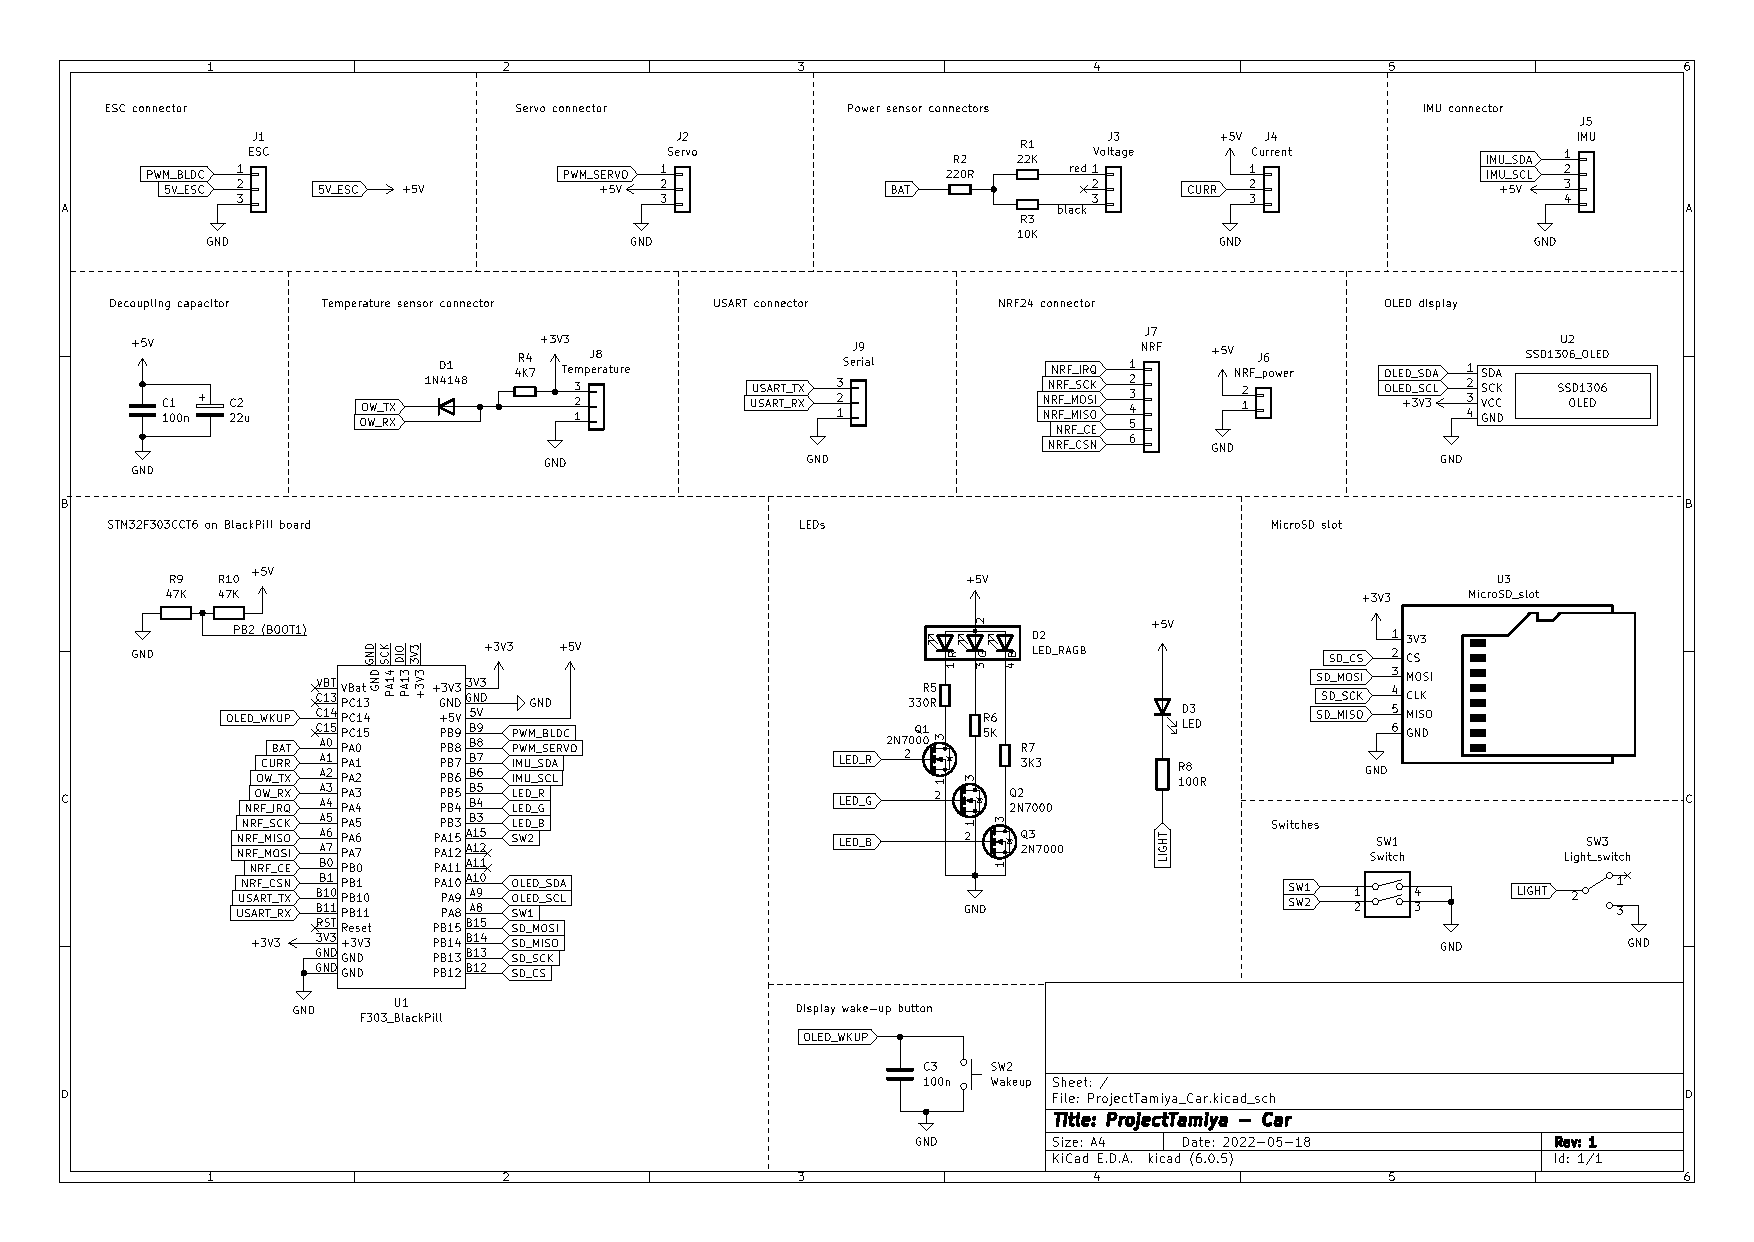
\includepdf[pages=1, angle=90, scale=0.78, offset=0 -45, pagecommand=\appendix{Schematics}]{fig/ProjectTamiya_Car_schematics.pdf}
\newpage
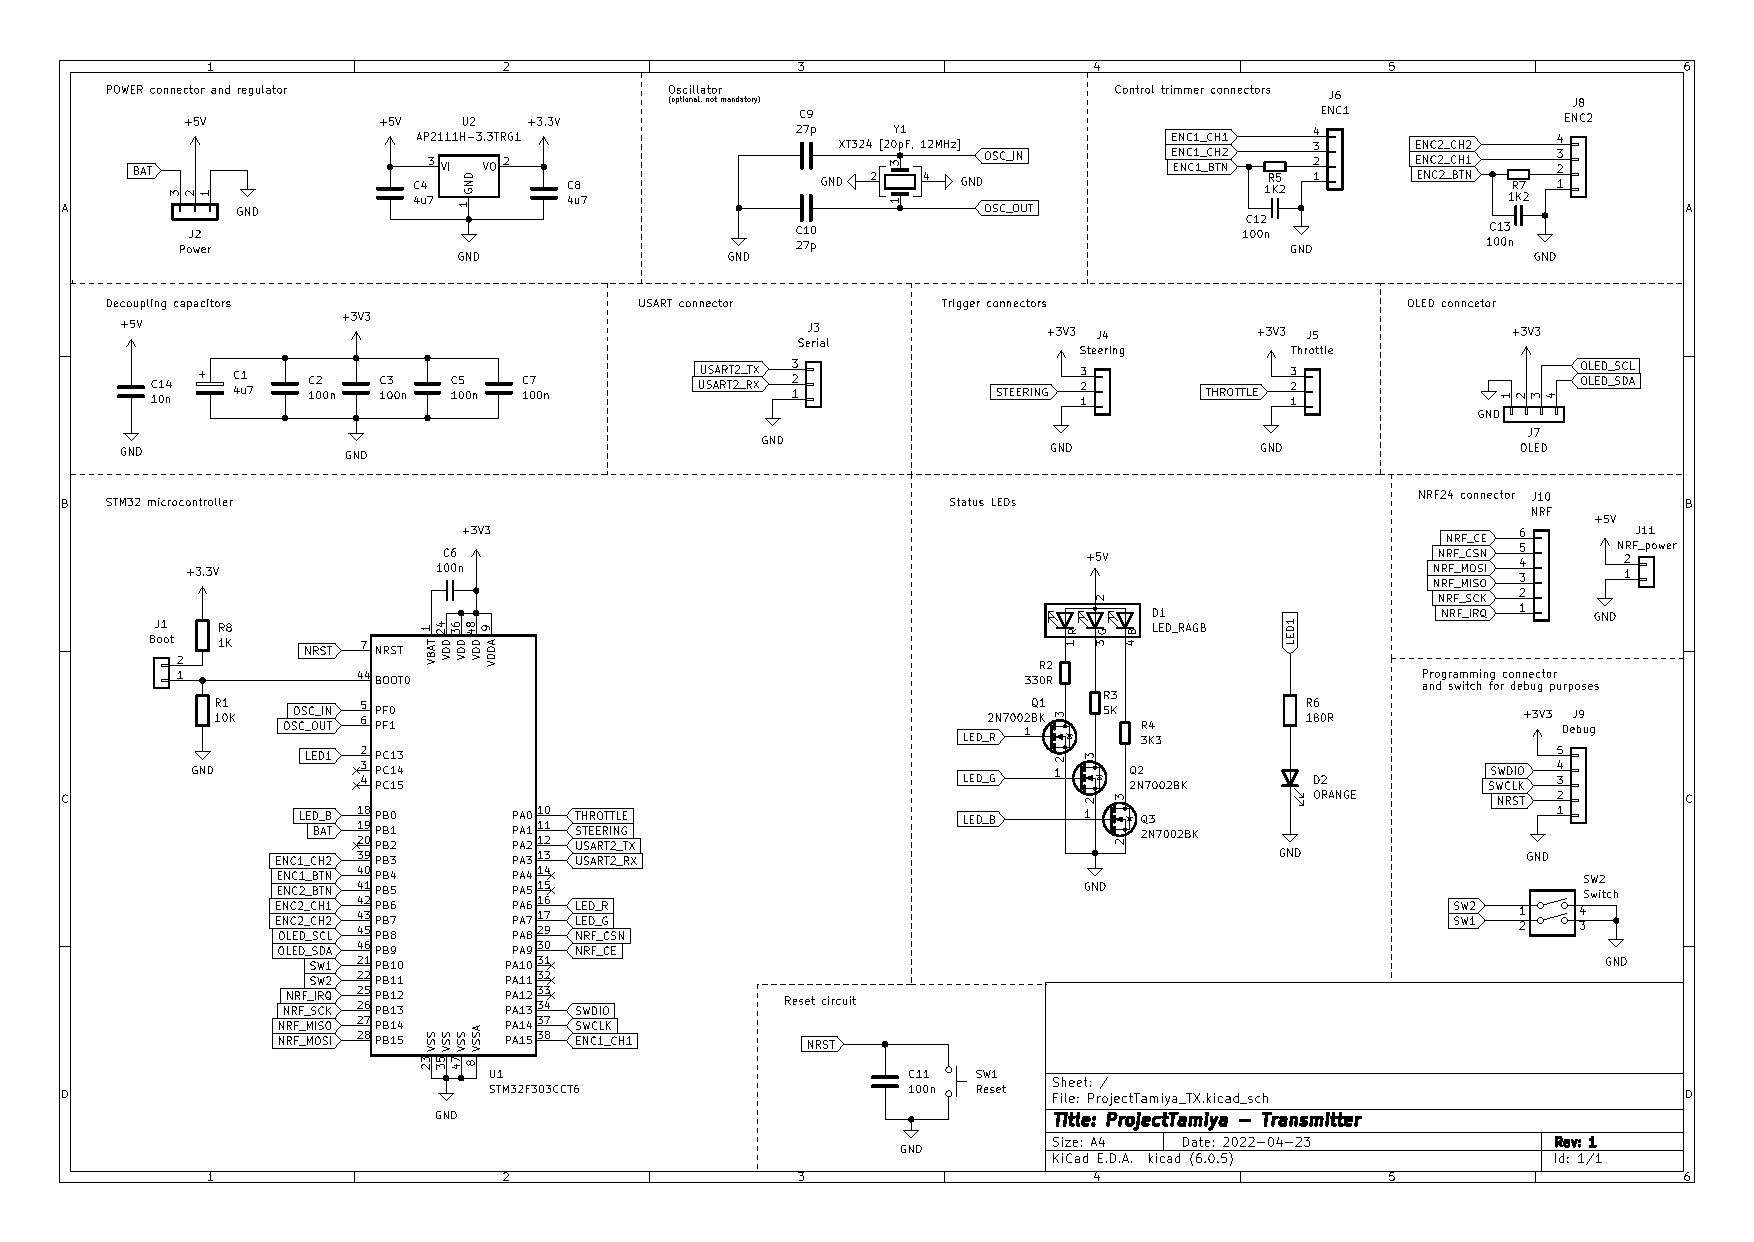
\includepdf[pages=1, angle=90, scale=0.78, offset=0 -20, pagecommand={}]{fig/ProjectTamiya_TX_schematics.pdf}

\newpage
\appendix{Supplementary material}
The attached DVD shares the same file structure as mentioned GitHub repository and is described below. Only the folders have been compressed into zip archives.

\begin{table}[h]
   \renewcommand{\arraystretch}{1.1}
   \centering
%    \caption{ARM Core utilization in STM32 family}
    \label{tab:abbrev}   
    \begin{tabular}{c c}
       \noalign{\hrule height 1.1pt}\noalign{\smallskip}
	   \bfseries File & \bfseries Contents\\[0.2em]
	\noalign{\hrule height 1.1pt}\noalign{\smallskip}  

Software.zip 			& source codes and drivers for both control applications, shared libraries \\
Hardware.zip 			& KiCad schematics and gerber files \\
3D\_printed\_parts.zip	& STL models for 3D printing \\
Logs.zip					& Two example logs in CSV format \\

       \noalign{\smallskip}\noalign{\hrule height 1.1pt}
    \end{tabular}
\end{table} 